\documentclass[]{article}

\usepackage{graphicx}

%opening
\title{Figures for  3-D printed oxygen devices}
\author{}

\begin{document}

%\maketitle

\section{figures}

\begin{figure}[H]
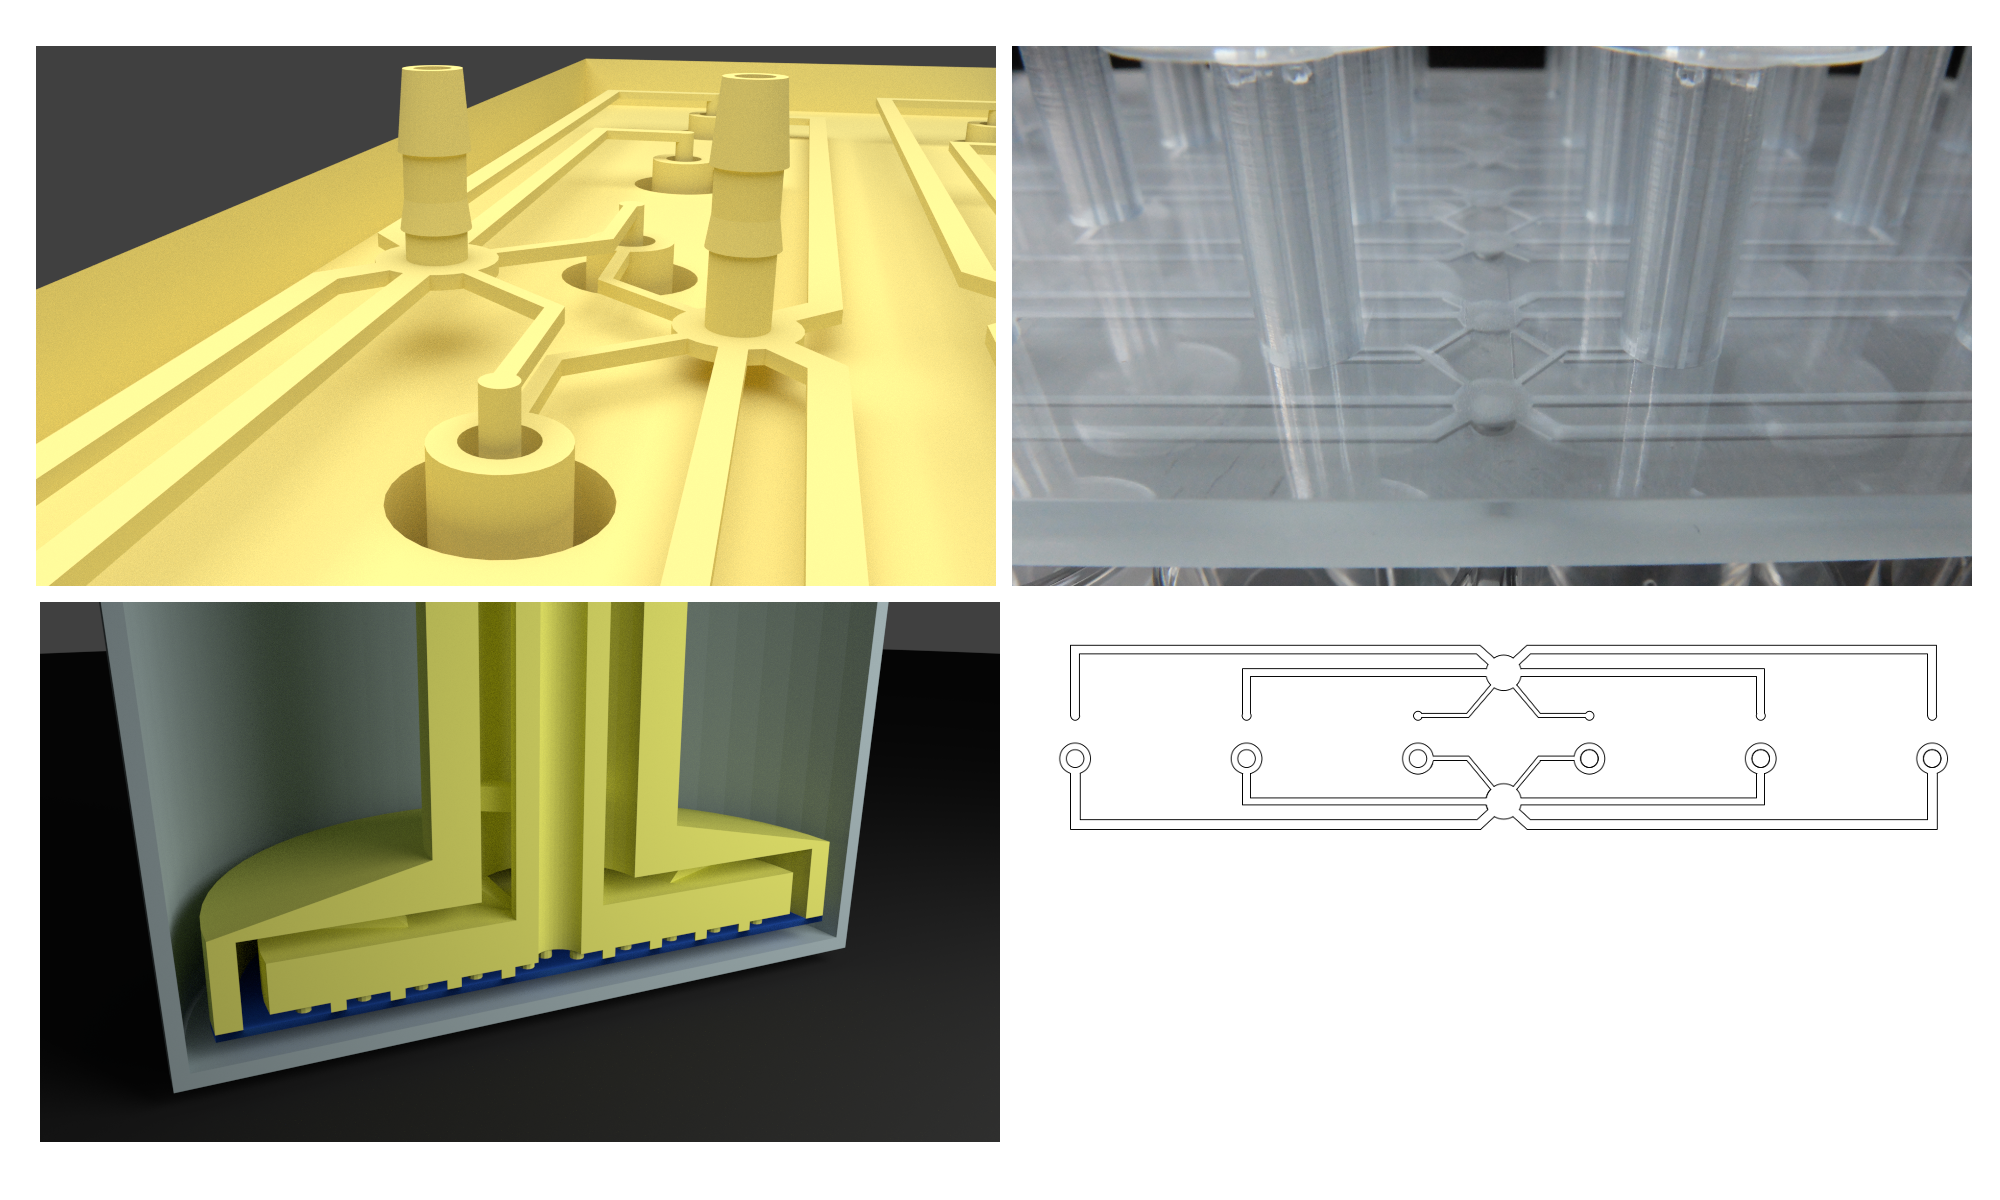
\includegraphics[scale=0.2]{fig1.png} 
\caption{
{\bf 24-well Insert Device.} A microfluidic network distributes gas flow from one hose barb input to 6 wells.
A 'Pipe with in a pipe' design delivers gas to the bottom of each well where it diffuses to the culture through an adhered PDMS membrane (blue-layer).  
The distribution network width of the channels in the distribution network are such that the flow rates are equalized to each well dependent on the path length.
}
\label{figure1}
\end{figure}

\begin{figure}[H]
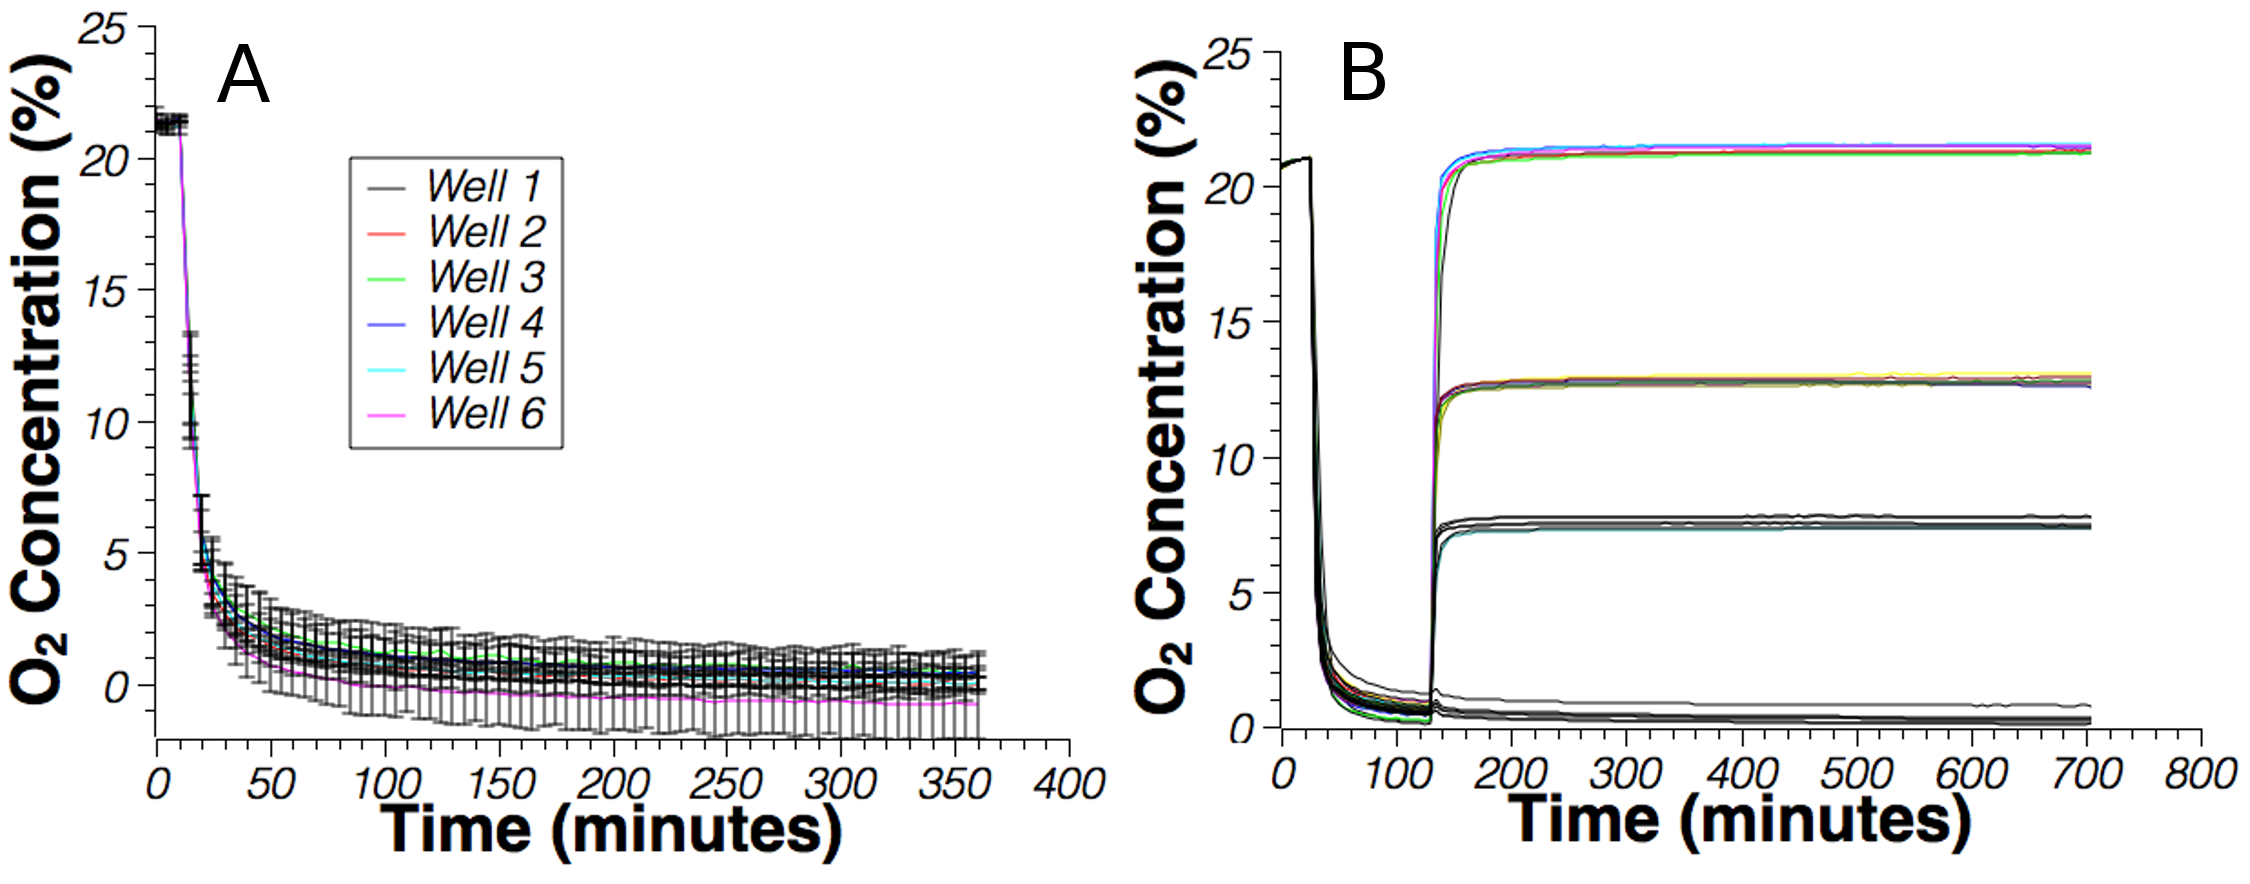
\includegraphics[scale=0.25]{fig2.png}
\caption{
{\bf Oxygen Characterization.}  Time course data of oxygen being evacuated from the culture area as 0\% oxygen gas is perfused through the device. Each 6 well row of the plate can be controlled independently.  
}
\label{figure2}
\end{figure}

\begin{figure}[H]
%\includegraphics[scale=0.2]{image.jpg} % remove for manuscript submission
\caption{
{\bf PCR Data.}  Not finished yet.  
}
\label{pcr-data}
\end{figure}

%\begin{abstract}

%\end{abstract}

%\section{}

\end{document}
